\documentclass[12pt,a4paper]{article}
\usepackage{color}%for coloured font
\usepackage[margin= 1 in]{geometry}%page margins
\usepackage{listing}%For item lists
\usepackage{graphicx}%To include graphics
%\usepackage{svg}
\usepackage{natbib}%bibliography
\usepackage[toc,page]{appendix}
\usepackage{setspace} \linespread {1}
\setlength{\parskip}{6pt}
\usepackage{array} %To get rid of paragraph indents
\setlength{\parindent}{0pt}
\usepackage{times}% Use times new roman font
\usepackage{amsmath}
\usepackage{booktabs}%for tables
%-------------------------------

\begin{document}
\begin{titlepage}
	\begin{center}
	\Huge{\textbf{Implementing monopod perching on a nano quadcopter}}
	\end{center}
\end{titlepage}


\setcounter{page}{2}

\tableofcontents

\pagebreak

\listoffigures

\pagebreak

\listoftables

\pagebreak
%-------------MAIN BODY-----------
\section{Introduction}
Small-sized VTOL drones, UAVs (Unmanned Aerial Vehicles) and UASs (Unmanned Aerial Systems) are currently one of the most sought after technologies in research and enterprises due to their small size and low power requirements. These systems provide the flexibility and manoeuvrability of a conventional helicopter whilst maintaining a fraction of its form factor. These characteristics have made drones an attractive tool for exploration or reconnaissance operations in highly dangerous, complex or inaccessible environments, but have also allowed for their introduction to the leisure market for applications such aerial photography. \textcolor{red}{DO I REALLY NEED THIS PARAGRAPH? IT MISSES OUT ON THE POINT}

Small-sized \textcolor{red}{VTOL} (Vertical Take-off and landing) drones ,UAVs (Unmanned Aerial Vehicles) and UASs (Unmanned Aerial Systems) currently face two major challenges which affect their applicability and practicality: Battery life and choice of landing surface. Battery life poses a considerable limitation in terms of flight time, inevitably setting a limit to the amount of data gathered during each flight operation, with flight times rarely exceeding 20-30 minutes. As in helicopters, these vehicles also require flat, stable and sufficiently wide surfaces for landing, and in many cases this can become an issue in applications such as rainforest canopy research or natural disaster zone reconnaissance operations.

-Talk about what others have done to assess the issue of short battery life
	
A significant amount of attempts at solving these issues involve a bio-inspired solution known as perching: When flying beings such as birds or insects do not need to stay airborne, they are able to land in locations such as power lines, posts or branches where they can rest and perform other tasks in the meantime. \cite{PerchTypes} compiles a comprehensive array of perching techniques currently investigated, which include chemical adhesion, suction cups, synthetic gecko skin, claws, microspines and electroadhesion.  The Biomimetics \& Dexterous Manipulation Laboratory at Stanford University have an extensive research record on the use of microspines to successfully achieve perching in ceilings and vertical surfaces in microquadrotors \cite{SCAMP} and small fixed-wing UAVs \cite{microspines}. Harvard University's Robobee \cite{robobee} makes use of electrostatic adhesion to allow an insect-sized drone to perch on a variety of surfaces. However, this technology has only been currently proven to work on very small-sized systems and scalability to larger  machines might be compromised by large power requirements. Worth noting as well are the works of \cite{bird} on the development of an avian-inspired passive perching mechanism and \cite{insect} for its insect counterpart, which, although more lightweight, only offers limited landing location flexibility.


-Comment on problems with their designs (high mass, very specific applications in terms of landing spot, extra battery needed, not being able to yaw, etc)

The vast majority of the exposed projects share a common flaw: They depend to some extent on the available landing surface area, necessary for mechanisms such as microspines to be satisfactorily deployed, which could render them ineffective in situations where a sufficiently large landing spot is not available. This limitation is mitigated in \cite{bird} by using a bird-like claw mechanism, but at the added cost of a heavier assembly which could severely affect active flight time in small-sized UAVs. Owing to this, it would be desirable to develop a platform light enough to be carried by a small-sized drone without significantly affecting flight time and manoeuvrability and which allowed it to perch on locations such as edges or other complex geometries where deployment of claw-like mechanisms would be difficult.


-Introduce the work by Hao Wang on one DOF quanser


A recent study investigated the feasibility of a novel technique termed "monopod perching" on a 3 degree-of-freedom Quanser helicopter for a single (pitch) axis of rotation with cascaded PID attitude control \cite{Hao}. With this method the weight of the drone is held by a single lightweight rod (figure \ref{fig1}), allowing the drone to perch on a single point while its motors operate at minimal power for balancing. This form of active perching would obviate the need for a sufficiently smooth/rough landing surface, and the quality of perching would be unaffected by the surface area of the landing location. Furthermore, yawing about its support axis for reorientation and/or data gathering in different directions would be possible, becoming a useful feature in reconnaissance missions.

\begin{figure}[h!]
\centering
 % \includegraphics[scale=0.5]{Fig1.pdf}
  \caption{Monopod perching drone \textcolor{red}{label the picture}}
  \label{fig1}
\end{figure}


-Describe what this paper is concerned with achieving


The aim of this paper is focused on the implementation of this technology on a Crazyflie 2.0 nano quadcopter, studying its feasibility and characterising its behaviour as a function of \textcolor{red}{monopod} length. The performance metrics will involve measurement of perching and hovering time, disturbance rejection and assessment of stability on various surfaces and geometries. The results obtained in this project will shed light on the capabilities and scalability of this approach, allow for the creation of PID tuning guidelines and aid identification of possible limitations. \textcolor{red}{MAYBE PUT STAGES OF FLIGHT HERE?}




\section{Experimental set-up and testing}
The Crazyflie 2.0 nano quadcopter was used as the test platform for this project. Its small size and high modularity made it an attractive choice, as well as its open-source code, which allows for extensive modifications to suit each application. A Crazyradio PA was used to communicate with the quadcopter, and development was performed in a Bitcraze virtual machine, built specifically for development of this quadcopter and freely available online.
	
\subsection{Dynamic model of drone}
-Show my dynamic model of the drone + equations. Show also expected max roll/pitch angles? Describe here the stick lengths that will be used as well.


A dynamic model of the drone was developed to be compared against experimental results, \textcolor{red}{finding approximate PID gains}, and identifying sensible monopod lengths. A nano quadrotor can be depicted as a central mass joined via massless and infinitely stiff arms to its motors. The monopod is modelled as an infinitely stiff, massless rod of length $L$, pivoting on a single point without friction. The maximum angle $\theta$ of inclination sustained on any axis (pitch/roll) for a given monopod length and quadcopter geometry will be achieved when the quadcopter is oriented such that all motors move within the axis's plane of rotation. Therefore, this angle will be dependent on the maximum thrust achievable by any pair of adjacent motors. Symmetry of the vehicle allows for a simplified 2D depiction of the dynamic model (Figure \ref{fig2}).

\begin{figure}[h!]
\centering
 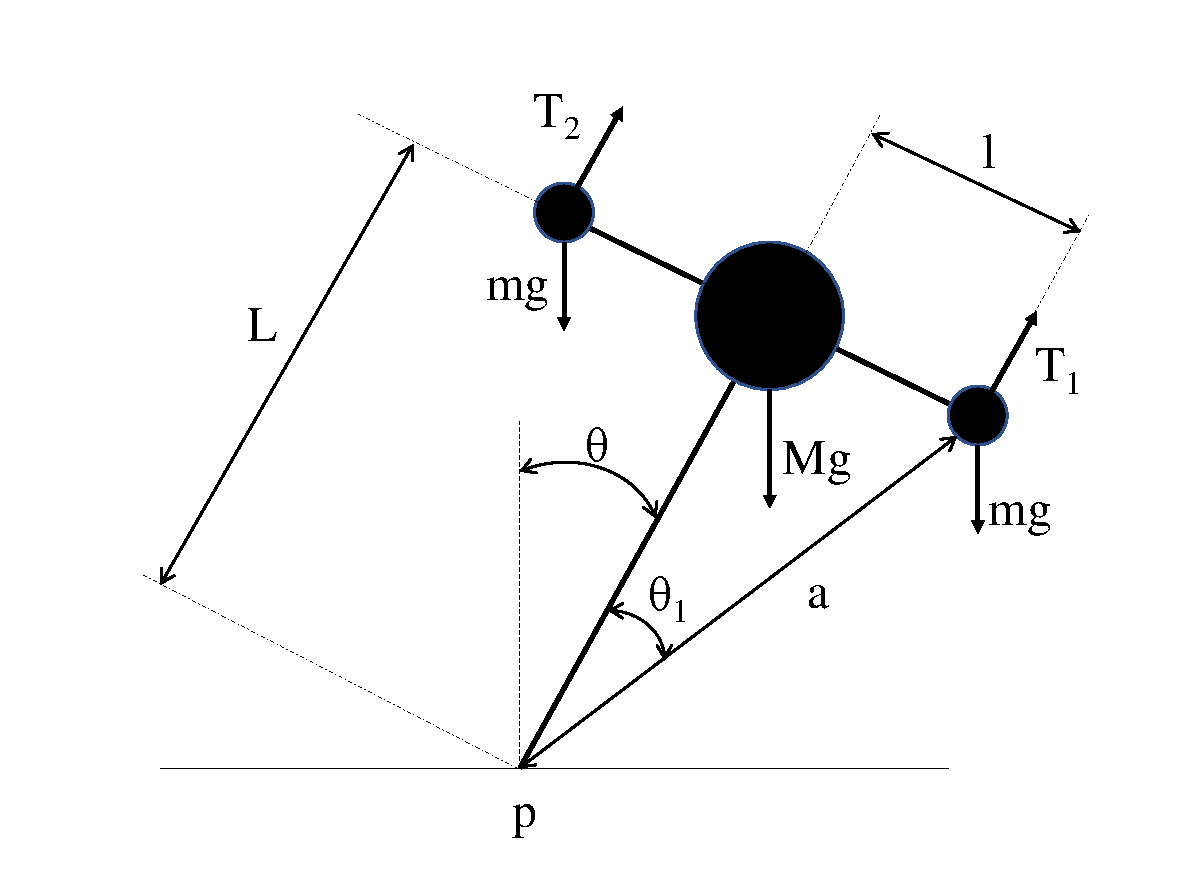
\includegraphics[scale=0.5]{dynamic_model.pdf}
  \caption{Dynamic model of perching drone. $T_1,T_2$ and $m$ represent thrust and mass from each pair of motors respectively, $L$ is length of the monopod, $M$ mass of the quadcopter, $l$ motor arm length and $\theta$ inclination angle}
  \label{fig2}
\end{figure}
Analysing moments about the perching point, $p$, the maximum inclination angle can be found by adopting a condition of equilibrium, where $\ddot{\theta} = 0$ (equation \ref{eq1}):
\begin{equation}
\begin{split}
mgasin(\theta + \theta_1) + MgLsin(\theta) + 
mgasin(\theta-\theta_1) \\
-T_{1}asin(\theta_1) + T_2asin(\theta_1) = 0
\end{split}
\label{eq1}
\end{equation}

Equilibrium at maximum tilt angle will take place when one pair of motors is operating at full thrust while the opposite pair remains at zero power. For consistency with figure \ref{fig2}, T$_{\text{2}}$ will be set to 0, and T$_{\text{1}}$ to full power. By considering the trigonometric identity

\begin{equation}
sin(A+B)+sin(A-B) = 2sin(A)cos(B)
\end{equation}

and rearranging, the maximum tilt angle $\theta_{max}$ can be found:

\begin{equation}
\theta_{max} = sin^{-1}\Big(\frac{T_1l}{2mgL + MgL}\Big)
\end{equation}

The parameters $T_{1}, l, m$ and $M$ were experimentally determined, and were recorded in \textcolor{red}{table \ref{table1}}. Figure \ref{fig3} shows $\theta_{max}$ as a function of monopod length $L$.


\begin{table}[h!]
\centering
\begin{tabular}{@{}ccccc@{}}
\toprule
T$_{1}$ {[}N{]} & l {[}m{]} & M {[}kg{]} & m {[}kg{]} & g {[}ms$^{-2}${]} \\ \midrule
0.05625         & 0.035     & 0.032      & 0.004      & 9.8               \\ \bottomrule
\end{tabular}
\caption{Experimentally determined parameters}
\label{table1}
\end{table}

\begin{figure}[h!]
\centering
 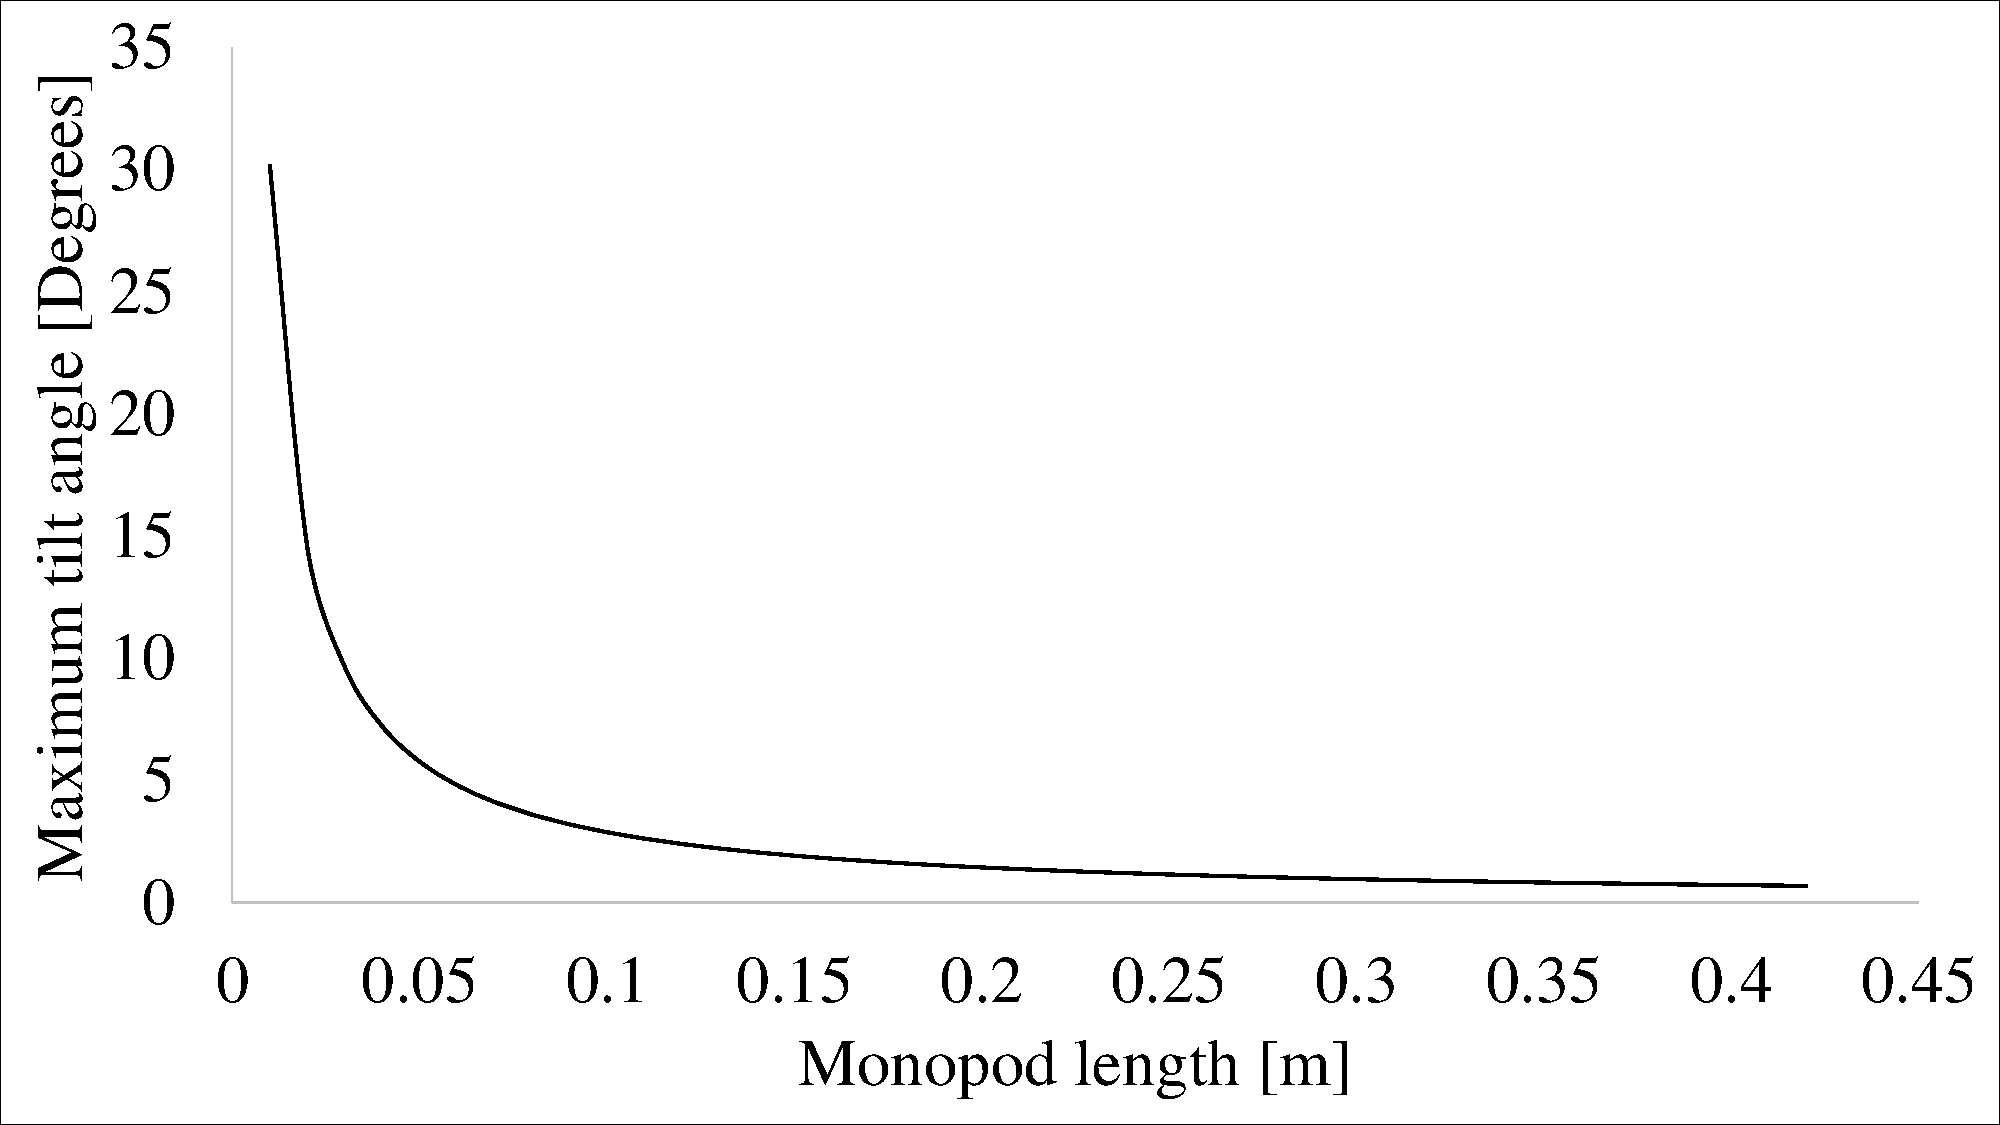
\includegraphics[scale=0.35]{TiltAngle.pdf}
  \caption{Maximum tilt angle $\theta_{max}$ as a function of monopod length}
  \label{fig3}
\end{figure}

In an effort to maintain the system sufficiently resilient to external disturbances, a maximum tilt angle of at least 2 degrees was decided upon. In order to maintain the infinitely stiff and massless monopod assumptions relevant, a maximum monopod length was assigned such that its weight would account for $<$5\% of the weight of the drone, and would not deflect more than 5 mm under cantilever loading with a mass equal to the weight of the drone. This set the maximum monopod length at $\approx$0.2 m. Monopod lengths of 1,2,3,4,6,8,10,12,14,16,18 and 20 cm were subsequently tested.

\subsection{Control structure and perching implementation}
The Crazyflie 2.0 nano quadcopter implements a cascaded PID control with Kalman filtering to respond to setpoints requested by the user. This consists of an outer loop running at low frequency which calculates the error between the desired and measured angle and outputs a desired angular rate to the inner loop. This inner loop is updated at a higher frequency and calculates the motor voltage required to induce a certain turning moment on the quadcopter, which translates into an angular rate which is compared against the desired angular rate. Figure \ref{fig4} illustrates the cascaded PID loop implementation.


\begin{figure}[h!]
\centering
 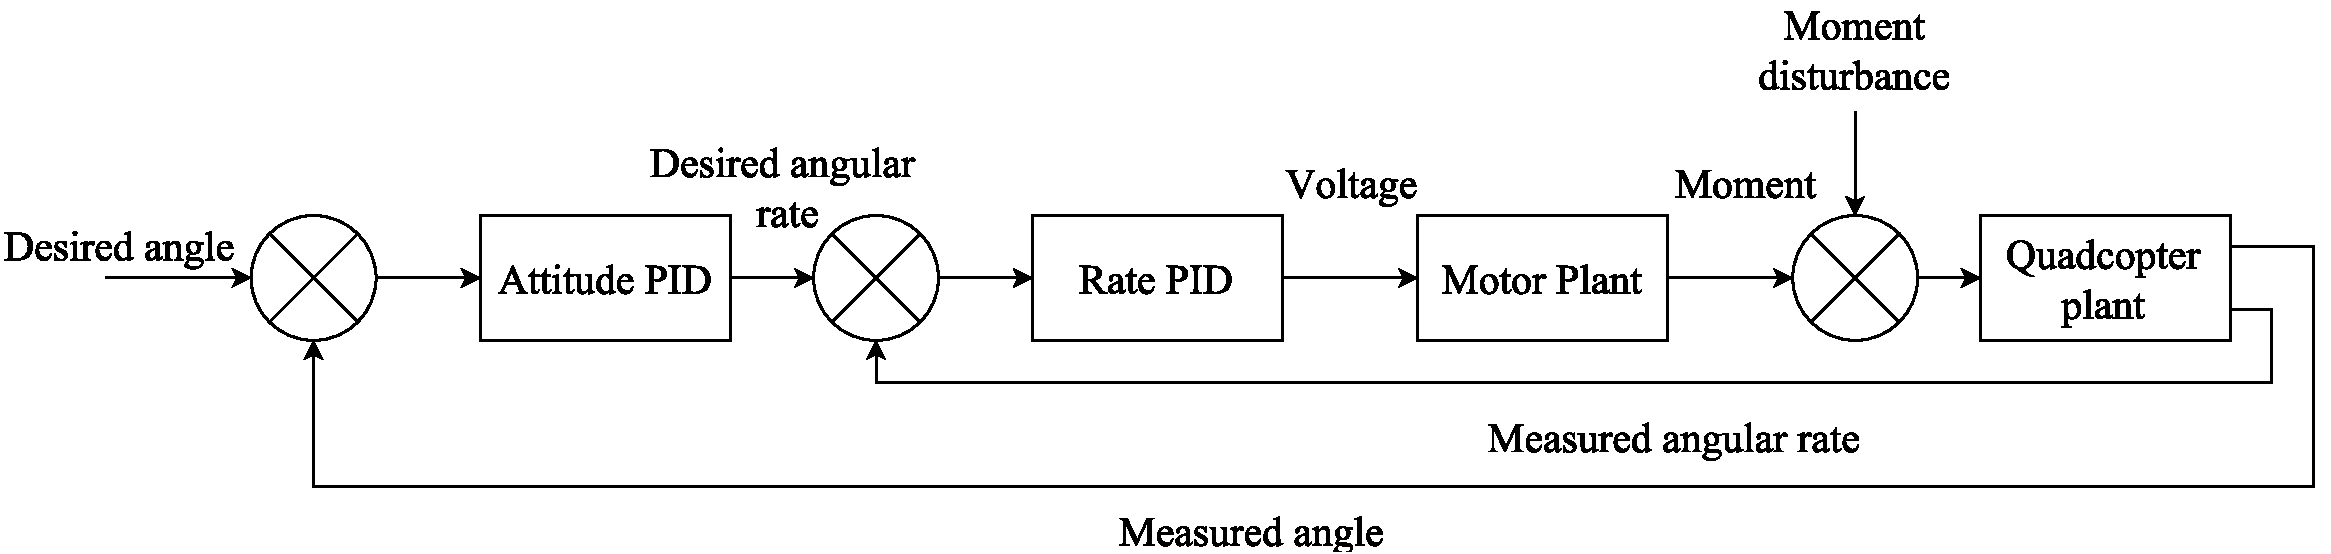
\includegraphics[scale=0.4]{Quad_PID.pdf}
  \caption{Cascaded PID controller on nano quadcopter}
  \label{fig4}
\end{figure}

Three independent cascaded PID control loops are used to control roll, pitch and yaw requests. The motor voltage requests from each axis are decoupled and linearly added together, allowing each PID controller to be independently tuned from the other two.

A PID controller takes the general form \cite{PID}

\begin{equation}
 u(t) = K_pe(t) + K_i\int_0^te(\tau)+K_d\frac{de(t)}{dt}
\end{equation}

Where $K_p, K_i, K_d$ are constant, non-negative gains, $e(t)$ is the error and $u(t)$ the output of the controller. A PID controller with constant gains can be used in linear, or weakly non-linear systems to closely approach optimal control. \cite{Hao} found in his study that a PID controller was suitable for implementation of monopod perching on a 1-axis experiment, as the tilt angles are generally very small ($<$14$^{\circ}$), and thus small angle approximations are applicable, allowing for linearization of the plant. However, furher non-linearities could arise from the motor plant, especially when rotating at low speeds, where the mapping between thrust and voltage may become non-linear.

The PID tuning approach will involve adjusting each axis separately. A typical approach CITE HERE involves first tuning the inner control loop for a zero angular rate reference until the quadcopter remains irrotational, but not necessarily upright. Finally, the outer loop will be tuned such that the quadcopter can be brought to the upright position, or to the correct yaw angle. This method proved ineffective for this application and its implications are further assessed in the discussion.

\begin{itemize}
\item Explain how cascaded PID is implemented in this drone(one PID for each axis). \textcolor{red}{what PID am I adjusting the parameters for? I need this info for the matlab model}. Explain that the idea is to get this PID controller to control the tilt of the drone, considering the tilt angles are small enough to linearise the problem.
\item Talk about the flight stages and which one we are mostly interested in on this paper (perching) Maybe leave this for the end
\end{itemize}

\subsection{Experimental set-up}
\begin{itemize}
\item Models of monopod/perching considered. p.8
\item p.13 test rig models considered/built and why they were used/modified/discarded.
\end{itemize}
A carbon fibre monopod was used to minimise weight impact while ensuring sufficient stiffness. A 3D-printed ABS plastic support was used to couple it to the quadcopter (Figure \ref{fig5}(a)). The tip of the monopod was sharpened to ensure single-point perching (Figure \ref{fig5}(b)). Care was taken to place the monopod underneath the center of gravity (CoG) of the quadcopter to minimise any imbalances. Any imbalances were corrected by shifting the position of the battery.

\begin{figure}[h!]
\centering
 %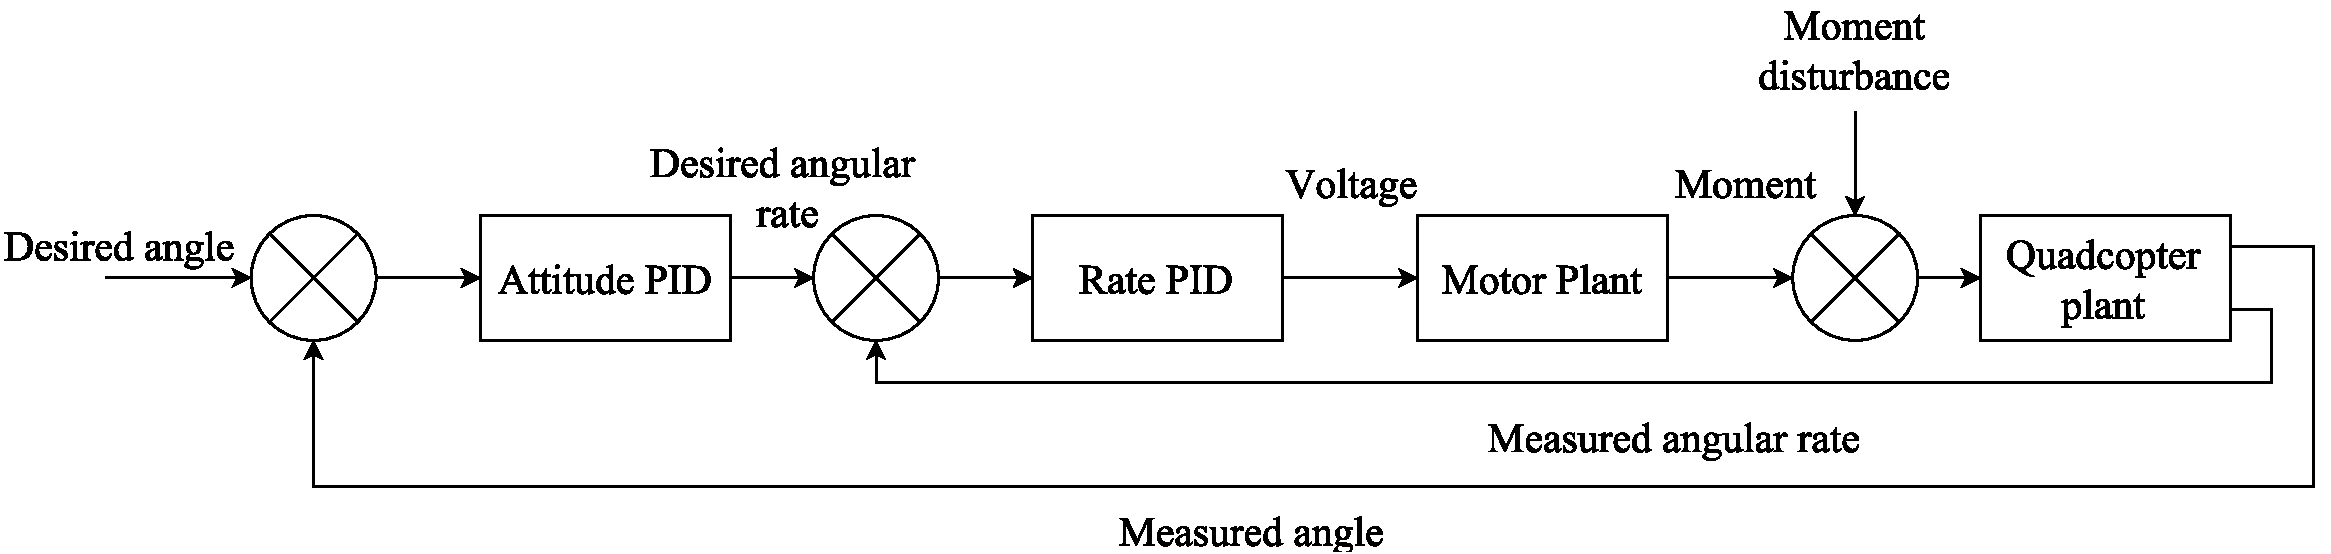
\includegraphics[scale=0.4]{Quad_PID.pdf}
  \caption{(a) Monopod assembly. (b) Detail of sharpened monopod tip}
  \label{fig5}
\end{figure}

A 1 DOF test rig was designed and built to adjust the three PID controllers (Figure \ref{fig6} (a)). A high-precision, low-friction bearing was used to minimise damping effects which would lead to excessively unresponsive PID gains, and the pivoting point was located at ground level to simulate true perching conditions. The damping on this test rig, together with the tuning method, was ineffective and a new test rig (Figure \ref{fig6}(b)) and tuning method (see section \ref{Results and discussion}) were used. The new hand-held test rig removes the friction component from the bearings and minimises air flow disruption by incorporating a long and thin handle. A small slot was created in an aluminium plate to avoid slip of the monopod.


\begin{figure}[h!]
\centering
 %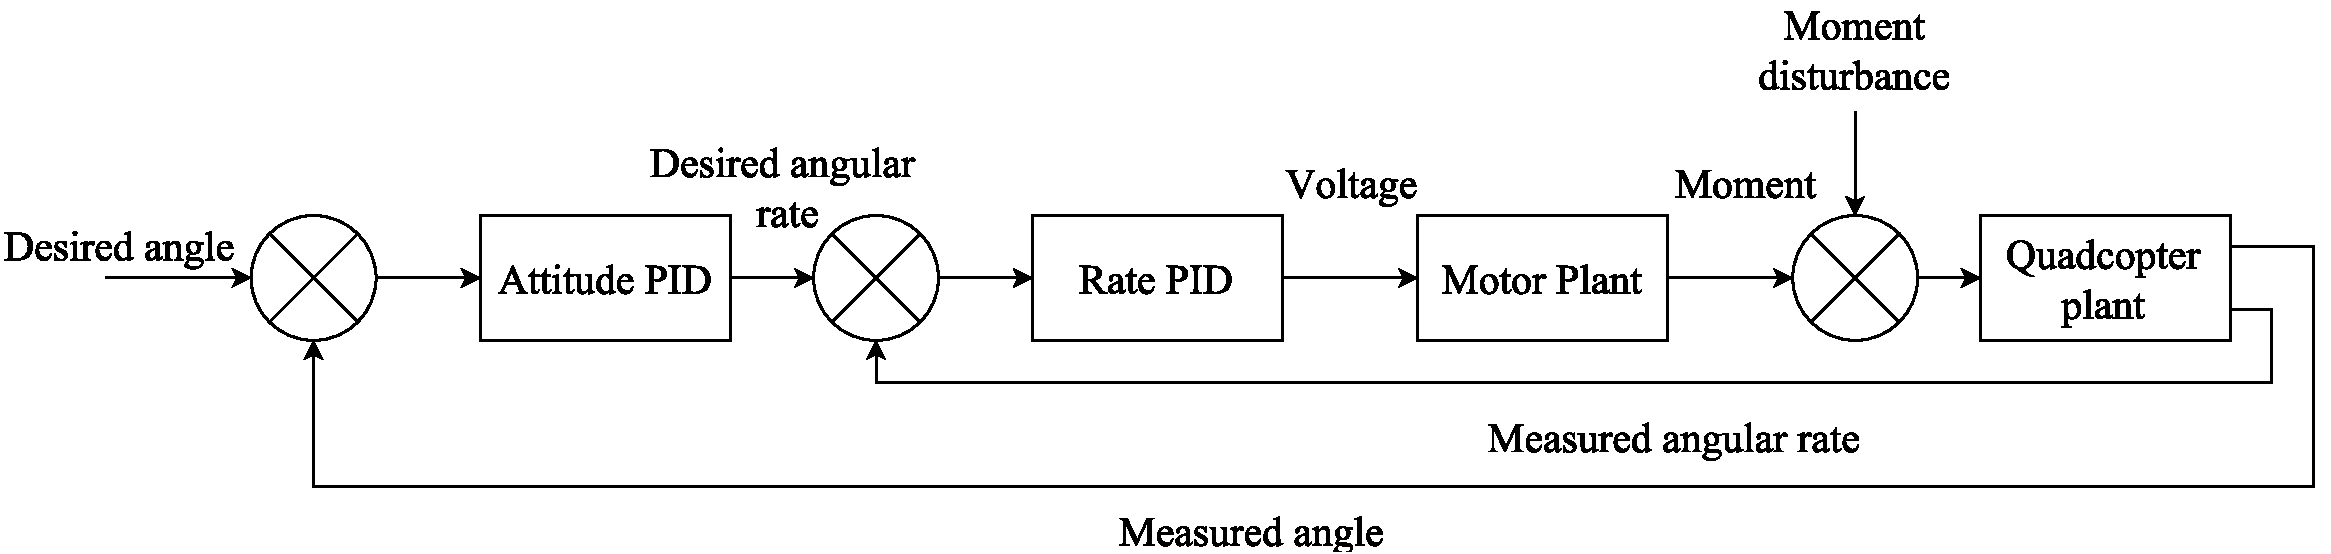
\includegraphics[scale=0.4]{Quad_PID.pdf}
  \caption{(a) Initial test rig. (b) Improved test rig}
  \label{fig6}
\end{figure}

\section{Results and discussion} \label{Results and discussion}
\subsection{PID controller tuning}
One of the most challenging aspects of this project involved determining suitable PID parameters for each monopod length: The very low mass and therefore inertia of the quadcopter made it very sensitive to small changes in CoG positioning and damping, greatly affecting the repeatability of results.

As previously explained, a 1 DOF test rig was initially employed to adjust roll, pitch and yaw PIDs. The following procedure was performed for each axis: Tune rate PID until quadcopter stayed in position and then tune attitude PID to maintain a desired angle. The base thrust component was kept at zero value, since the weight of the drone is already held by the monopod and the base thrust does not contribute to stabilisation.

This procedure resulted in K$_p$ and K$_i$ gains of the order of 10$^5$ for the rate PID, and very low gains for the attitude PID, as well as K$_d$ gains. The yaw PID, however, yielded much lower values. All parameters for a 8 cm monopod are compiled in \textcolor{red}{table \ref{table2}}. 

A strange behaviour was observed when the quadcopter was located on various surfaces to assess the efficacy and robustness of perching: On surfaces with significant damping, such as human skin, the quadcopter would remain consistently upright. On slippery surfaces, it would drift along the surface plane while remaining balanced. However, when the drone was located on surfaces with very low friction and where it was not possible to drift, it would instantly fall \textcolor{red}{(Show picture of slot in aluminium plate?)}. This phenomenon was initially believed to be due to a slightly incorrect location of the CoG. However, this hypothesis was later disproved by performing balancing experiments on the 1 DOF test rig, and noting that the quadcopter fell with a different orientation each time. Figure \ref{fig7} illustrates the behaviour under three different scenarios: 1 DOF test on test rig, test on slippery surface and test on low friction surface with restricted movement on surface plane.


\begin{figure}[h!]
\centering
 %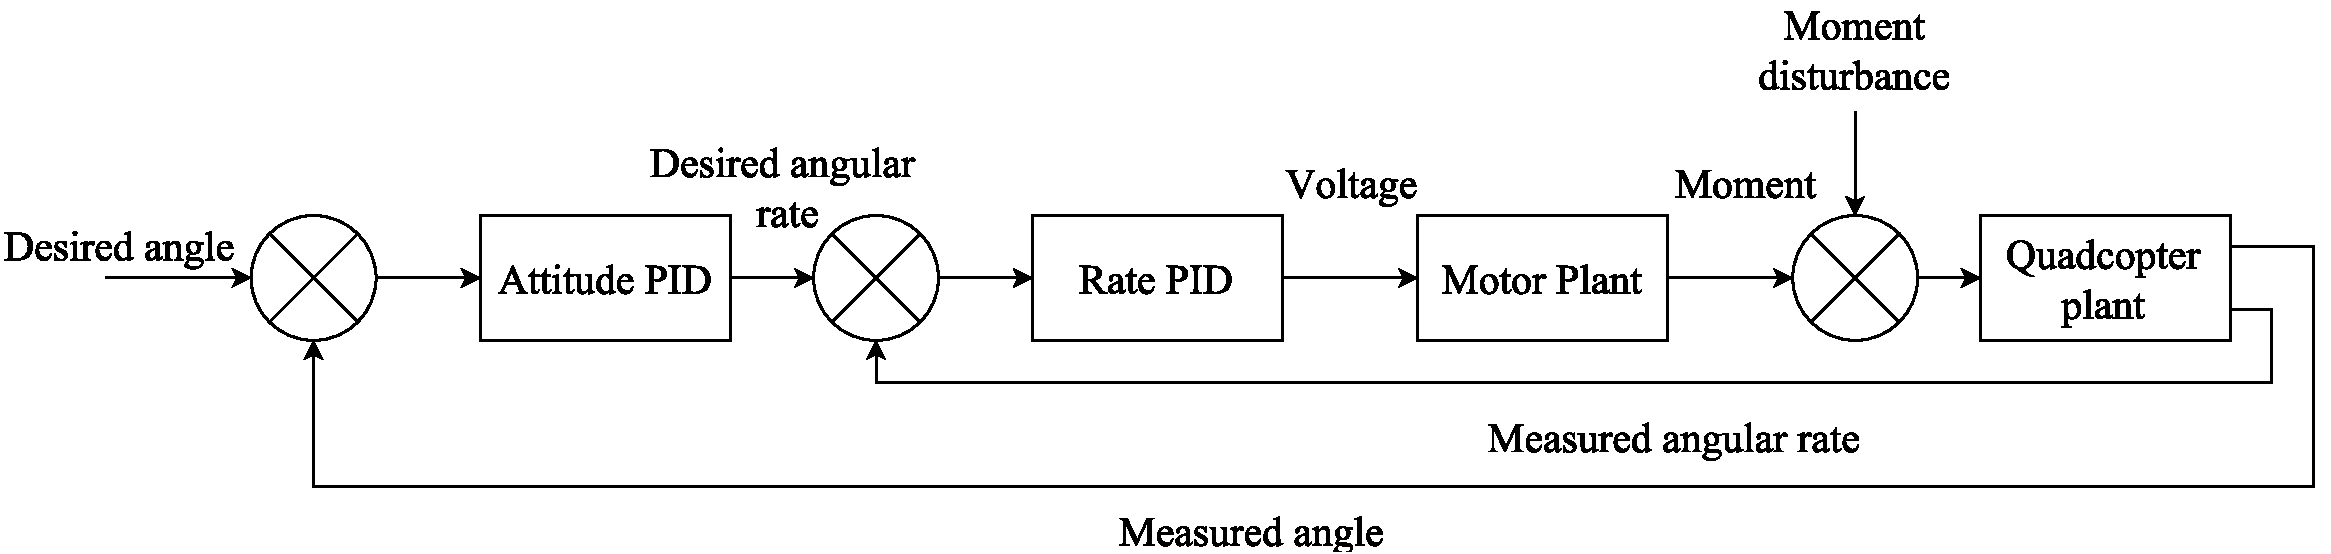
\includegraphics[scale=0.4]{Quad_PID.pdf}
  \caption{Roll, pitch and yaw angles on: (a) 1 DOF test on rig, (b) slippery surface, (c) test on low friction surface with restricted movement on surface plane}
  \label{fig7}
\end{figure}

A second hypothesis was devised, attributing this instability to the unusually high gains found, and, more crucially, the tuning method and test rig used. It was observed that the motors span either at zero or full speed, even for inclinations as small as 0.01$^{\circ}$ (Figure \ref{fig8}(a)). This, and the fast and violent vibrations about 0$^{\circ}$, suggested that the PID gains found were far from optimal. An assessment on the damping of the 1 DOF test rig was performed by letting it freely fall with no thrust input, and this was compared to a free fall without test rig (Figure \ref{fig8}(b)). The results obtained suggested that the 1 DOF test rig was significantly modifying the dynamics of the system, and a second test rig was designed to overcome these limitations (Figure \ref{fig6}(b))


\begin{figure}[h!]
\centering
 %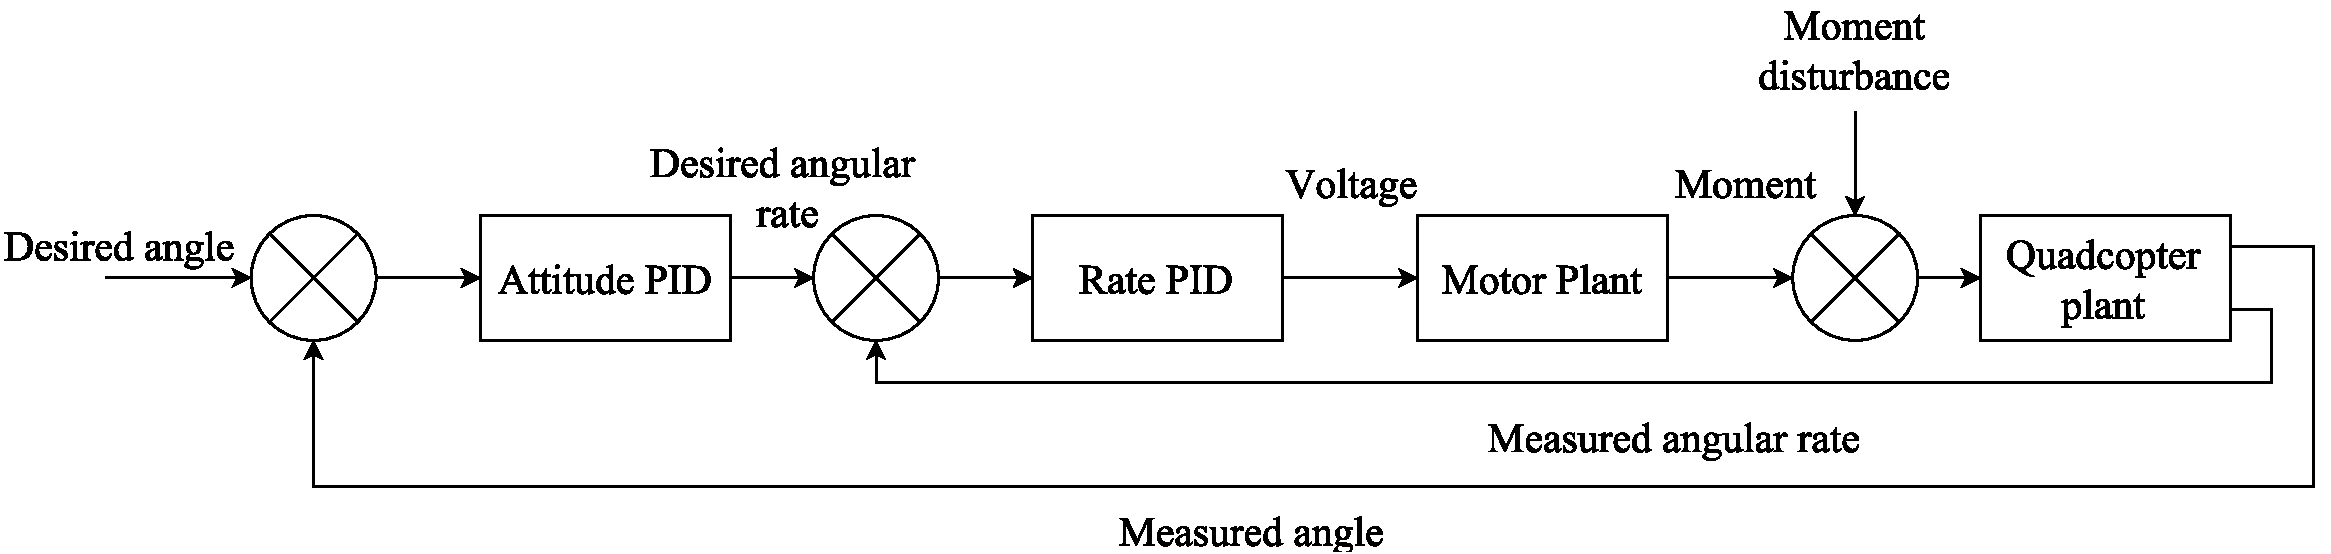
\includegraphics[scale=0.4]{Quad_PID.pdf}
  \caption{(a) Motor speed plot, (b) Free fall comparison on 1 DOF test rig and no test rig for damping assessment}
  \label{fig8}
\end{figure}

The most obvious limitation of this new test rig was that 1 DOF PID adjustment was not possible. However, since the controllers for each axis are decoupled, the symmetry of the quadcopter allowed for both roll and pitch control loops to be tuned simultaneously using the same parameters for both axes. The yaw controller also had to be enabled to avoid uncontrolled spinning of the quadcopter, which would eventually unsettle it and fall. A desirable tuning goal was to balance the quadcopter using mainly proportional gains to avoid integrator build-up in cases of sustained disturbances, which would cause the drone to remain unstable for a certain time until this term decreased sufficiently. This was the case with the old gains, and many times the controllers would have to be fully reset after a fall due to the very large integral gain that had accumulated.

After extensive trials, it was found that balancing the quadcopter on rate mode was not possible: The K$_p$ and K$_i$ terms were so large that motor saturation would cause them to simply turn either at zero or full speed, as was previously the case, but still fall. 

A different approach was used and the attitude PID gains were given a value of 1 each to aid in balancing. This allowed for much lower PID parameters to be determined, with an order of 10$^3$ for roll and pitch, subsequently resulting battery consumption. Final PID gains for a 8 cm monopod are compiled in table \ref{table2}. 

\begin{itemize}
\item table with PID parameters here
\end{itemize}

While performing preliminary endurance tests to assess how long perching could be sustained for on a single charge, another strange phenomenon was observed: On some occasions, the drone would suddenly become highly unstable and fall, with no influence from external disturbances or presence of imbalances in the drone. Figure \ref{fig9}(a) illustrates this behaviour: preceding the instability, no external disturbances have affected the quadcopter, yet the pitch and roll angles grow unbounded. This was initially attributed to sudden connectivity losses between the on-board controller and the pc client. However, subsequent tests verified that this was not the cause of falling. Further balance and external disturbance verifications were performed, but once again were found not to be the causes.

The cause of falling was finally attributed to the yaw controller: Yaw control was thought to be only necessary to avoid uncontrolled spinning, so a very rough adjustment, with oscillations of $\pm$20$^{\circ}$ was initially performed to focus attention on data gathering mainly related to pitch and roll. The unsettling was believed to happen when all pitch, roll and yaw were at their maximum amplitudes at the same time: The yaw controller would exert a fast turning moment, causing the quadcopter to quickly rotate about its monopod axis, changing roll and pitch angles a the same time. These fast changes would not allow the motors to respond fast enough to these changes due to their own inertia, eventually causing the drone to fall. The yaw PID was then readjusted, and an oscillation of $\pm$0.5$^{\circ}$ was found to be small enough to eliminate this phenomenon.


\begin{figure}[h!]
\centering
 %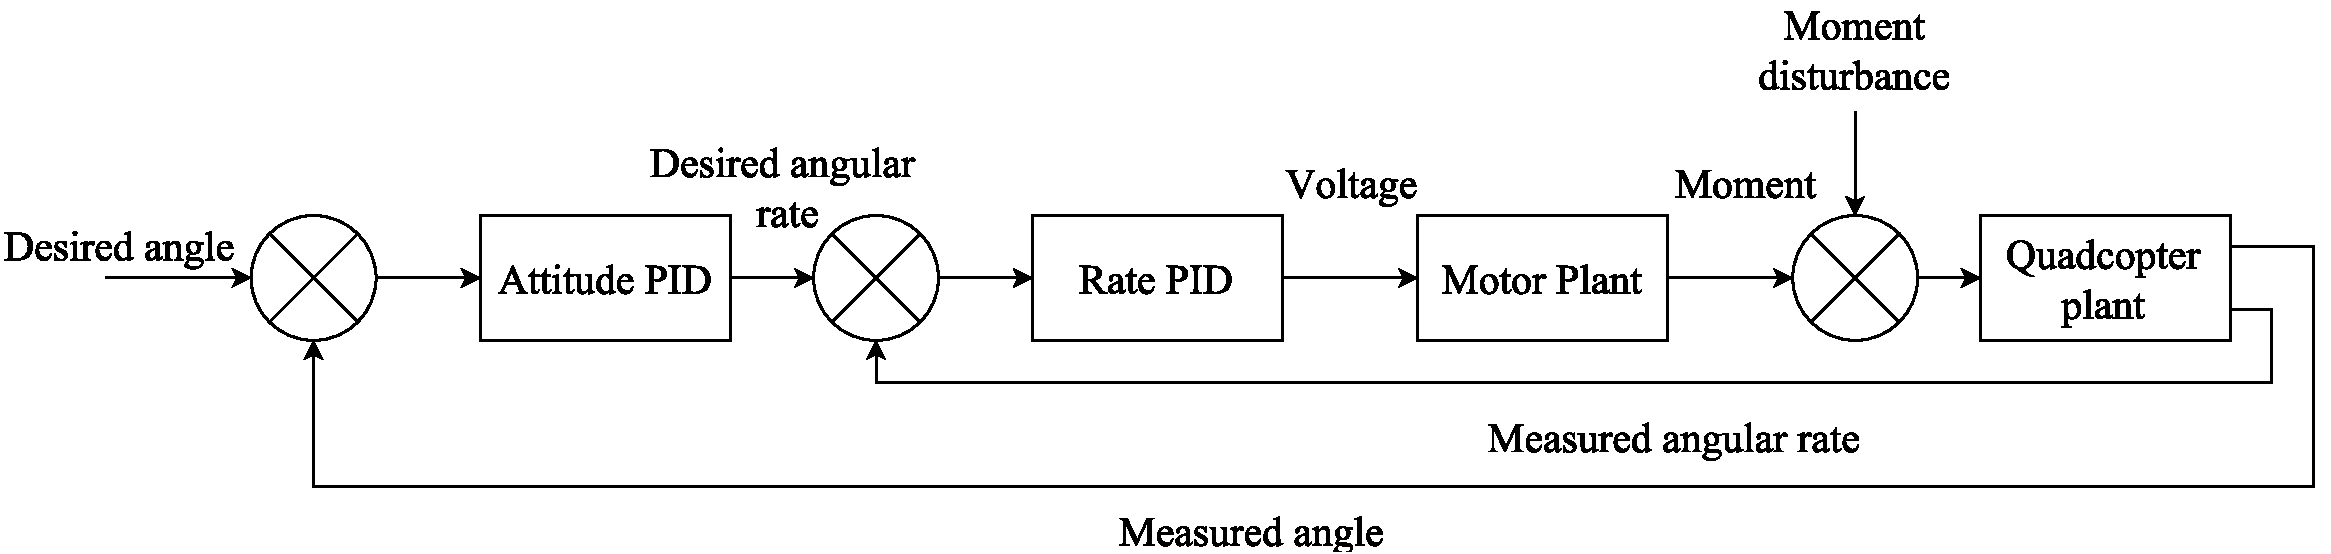
\includegraphics[scale=0.4]{Quad_PID.pdf}
  \caption{(a) Sudden unsettling of quadcopter, \textcolor{red}{(b) Detail of yaw angle at the point of unsettling }}
  \label{fig9}
\end{figure}



\subsection{Characterisation and analysis of perching quadcopter}

\begin{figure}[h!]
\centering
 \includegraphics[scale=0.23]{Perch_Time.pdf}
  \caption{(a) Perch time and hover time as a function of $L/l$, (b) Pareto chart with total operation time as a function of $L/l$ }
  \label{fig10}
\end{figure}

\begin{figure}[h!]
\centering
 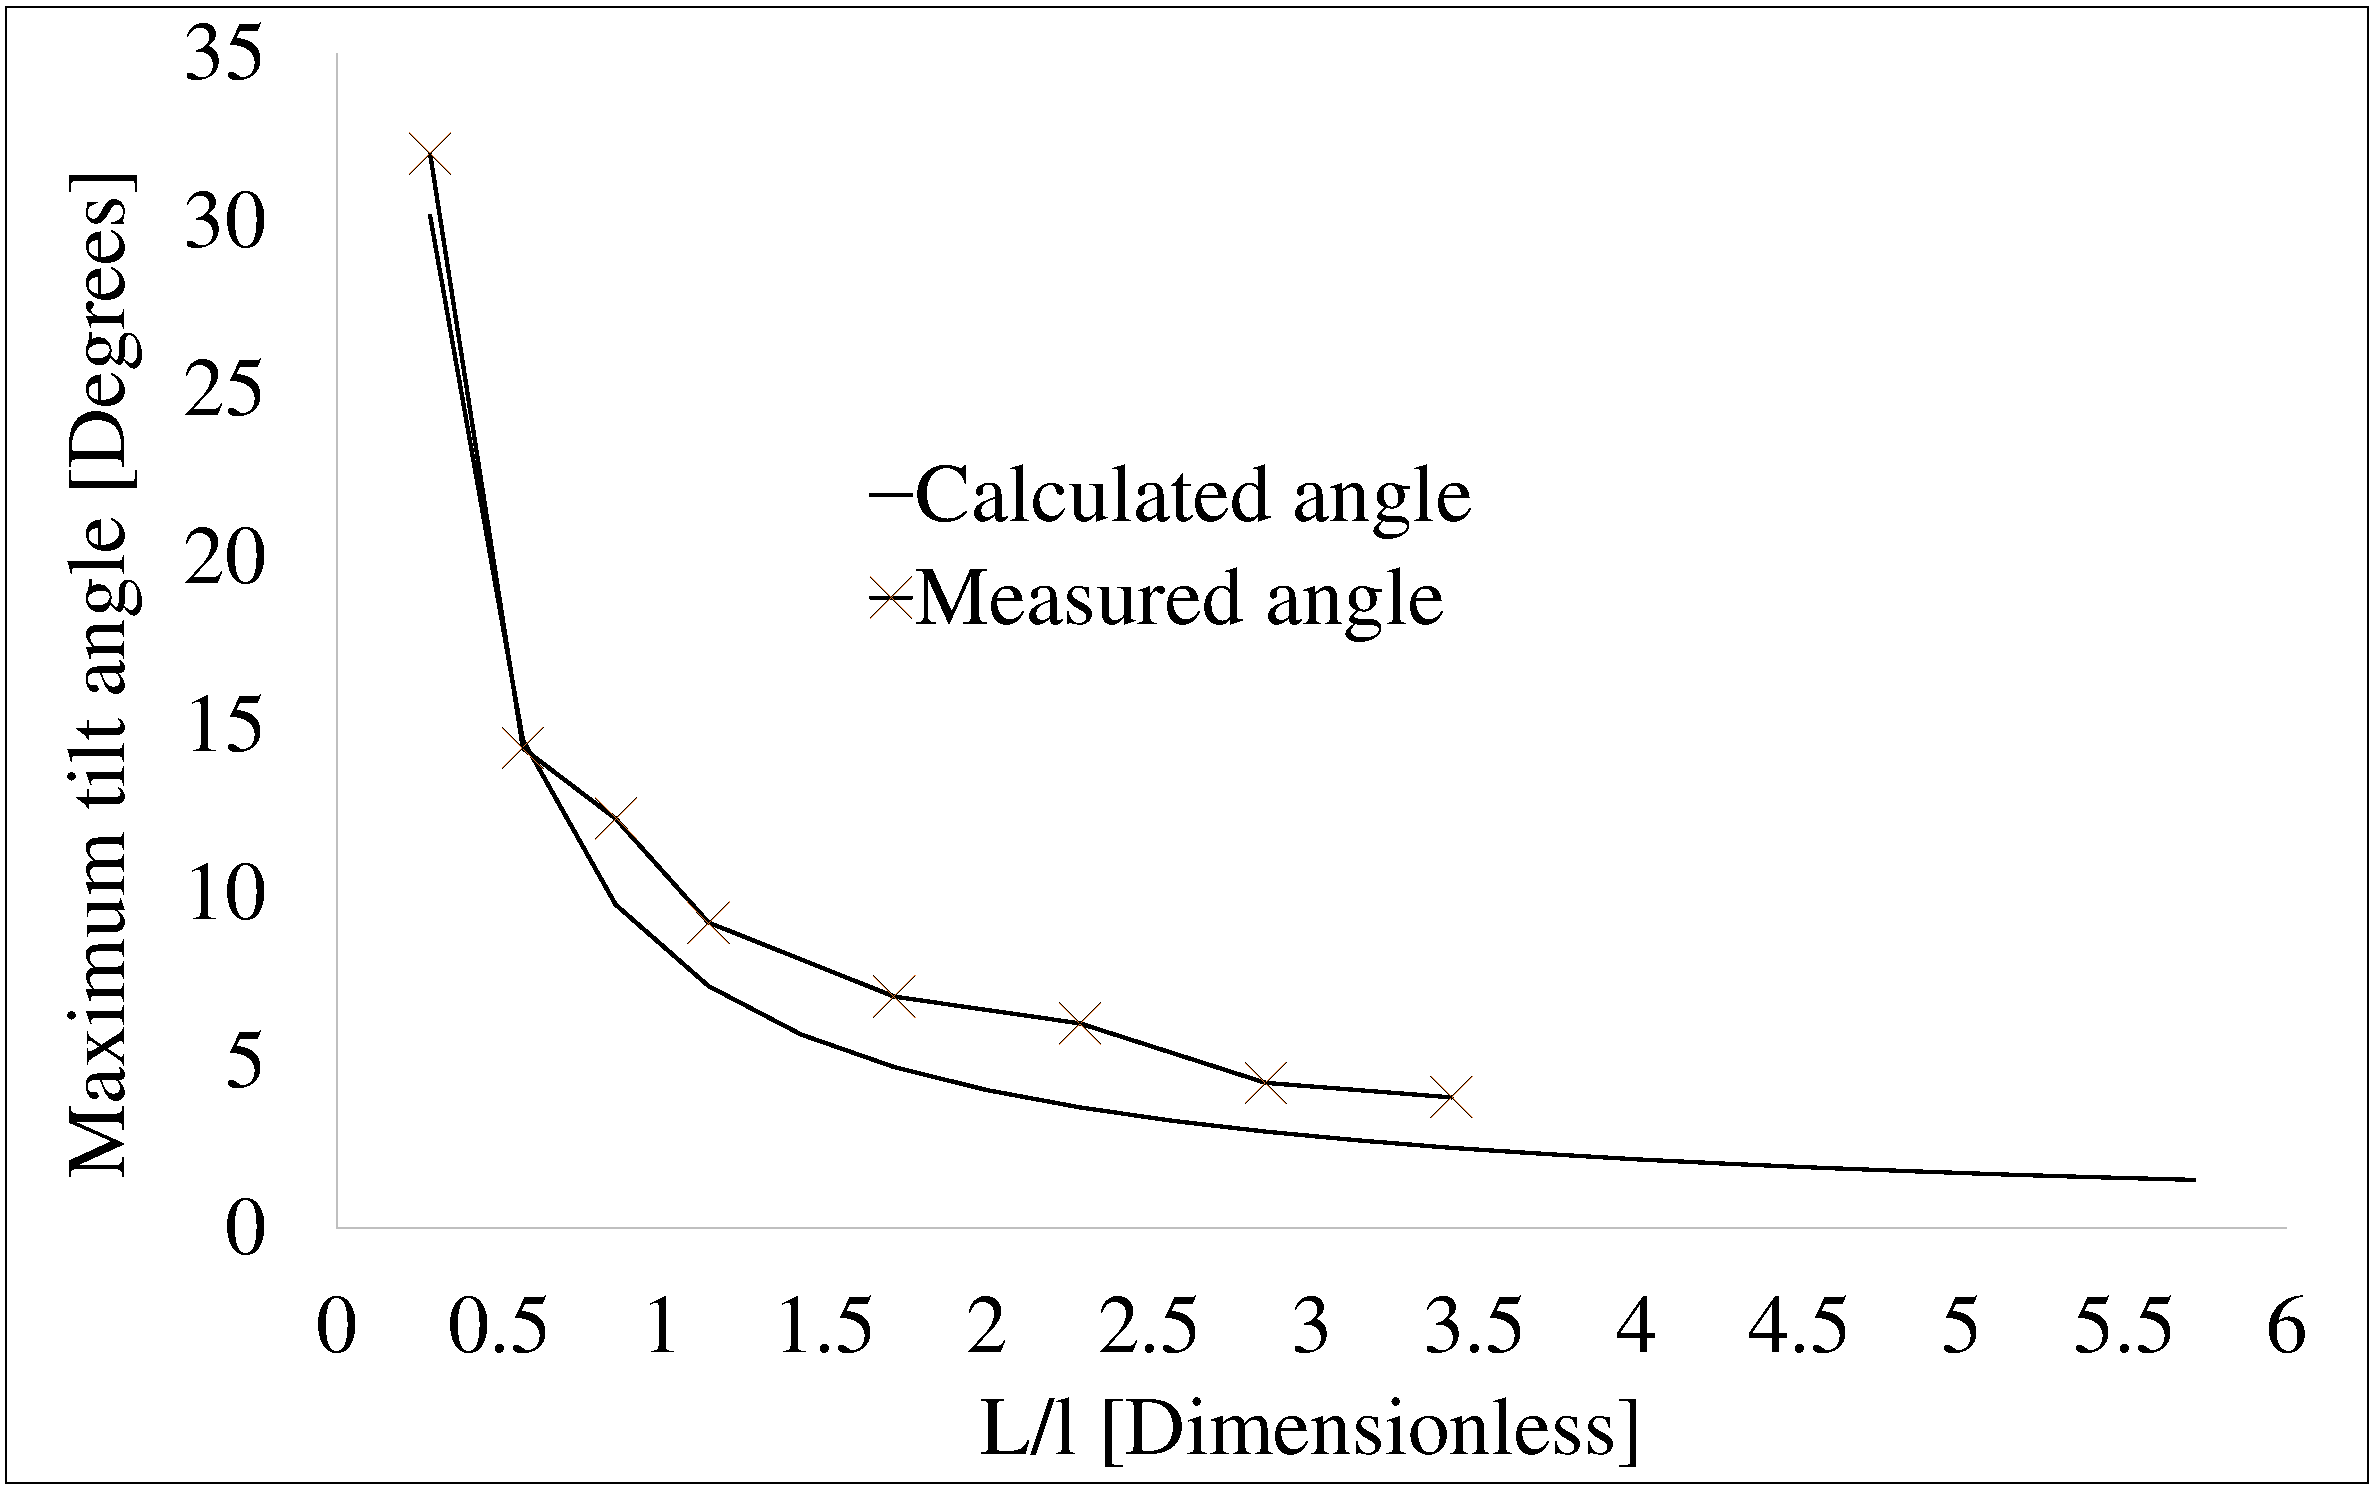
\includegraphics[scale=0.3]{TiltAngle_2.pdf}
  \caption{Measured and calculated maximum tilt angles as a function of $L/l$}
  \label{fig11}
\end{figure}

\begin{figure}[h!]
\centering
 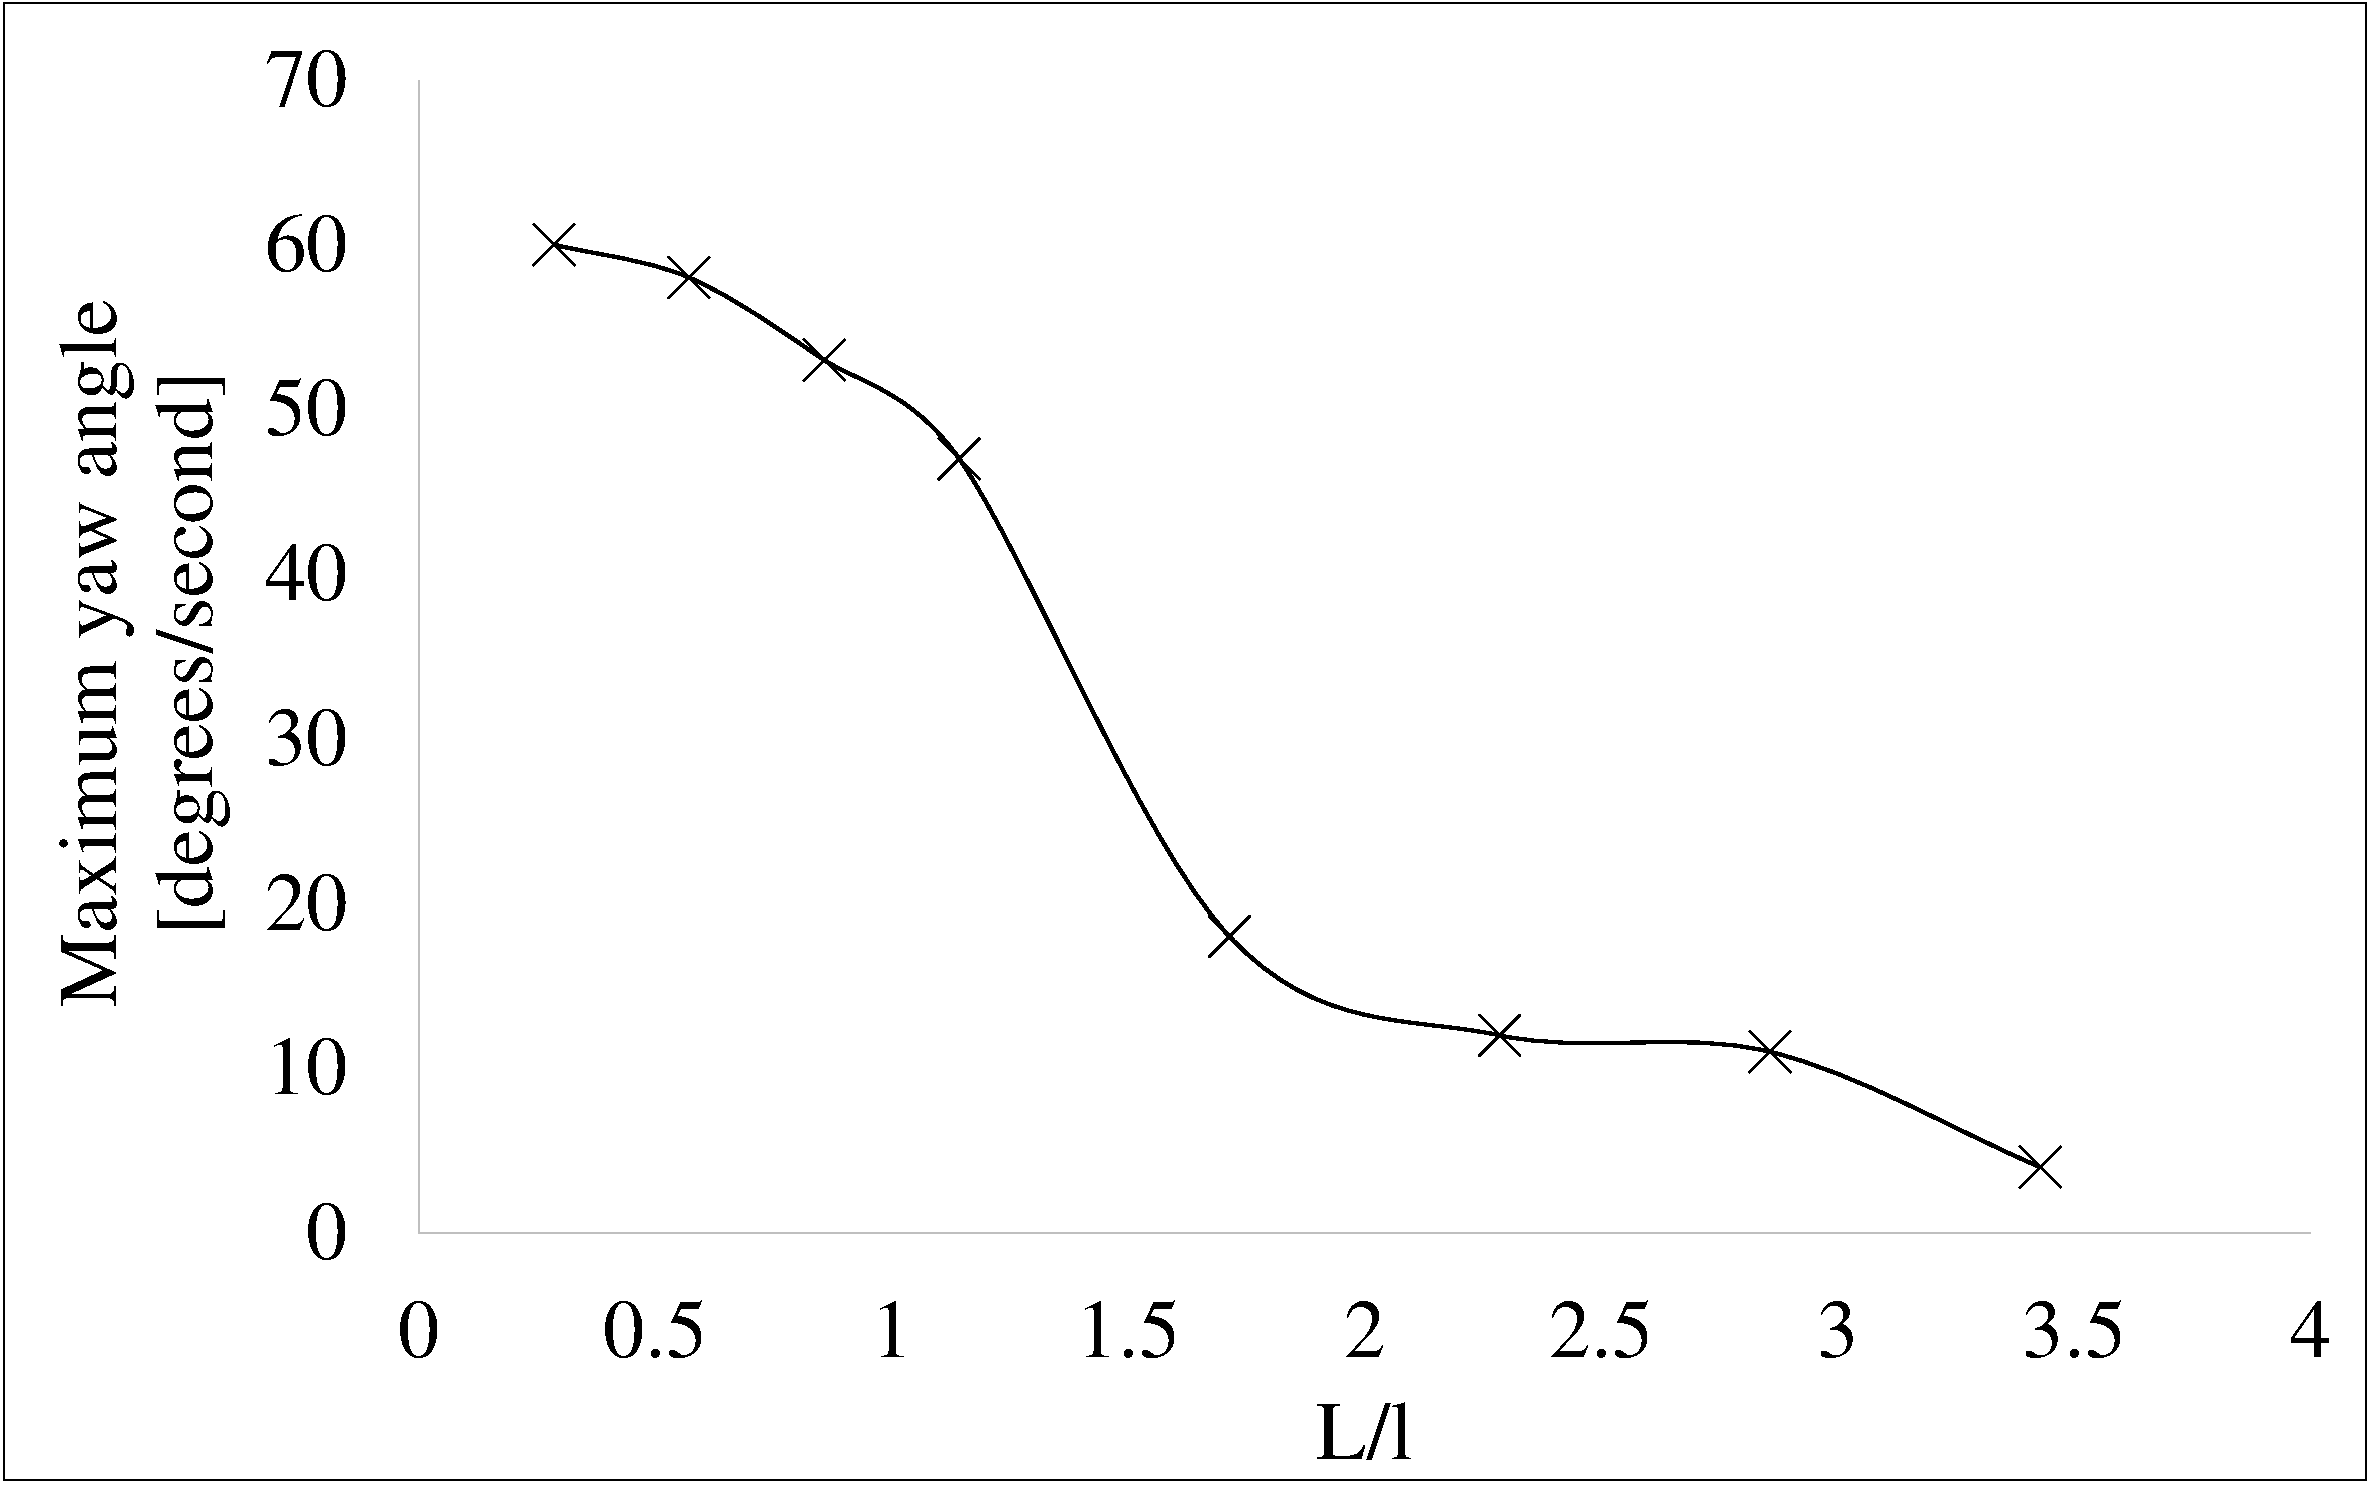
\includegraphics[scale=0.3]{Yawrate.pdf}
  \caption{Maximum yaw rate as a function of $L/l$}
  \label{fig12}
\end{figure}

\begin{figure}[h!]
\centering
 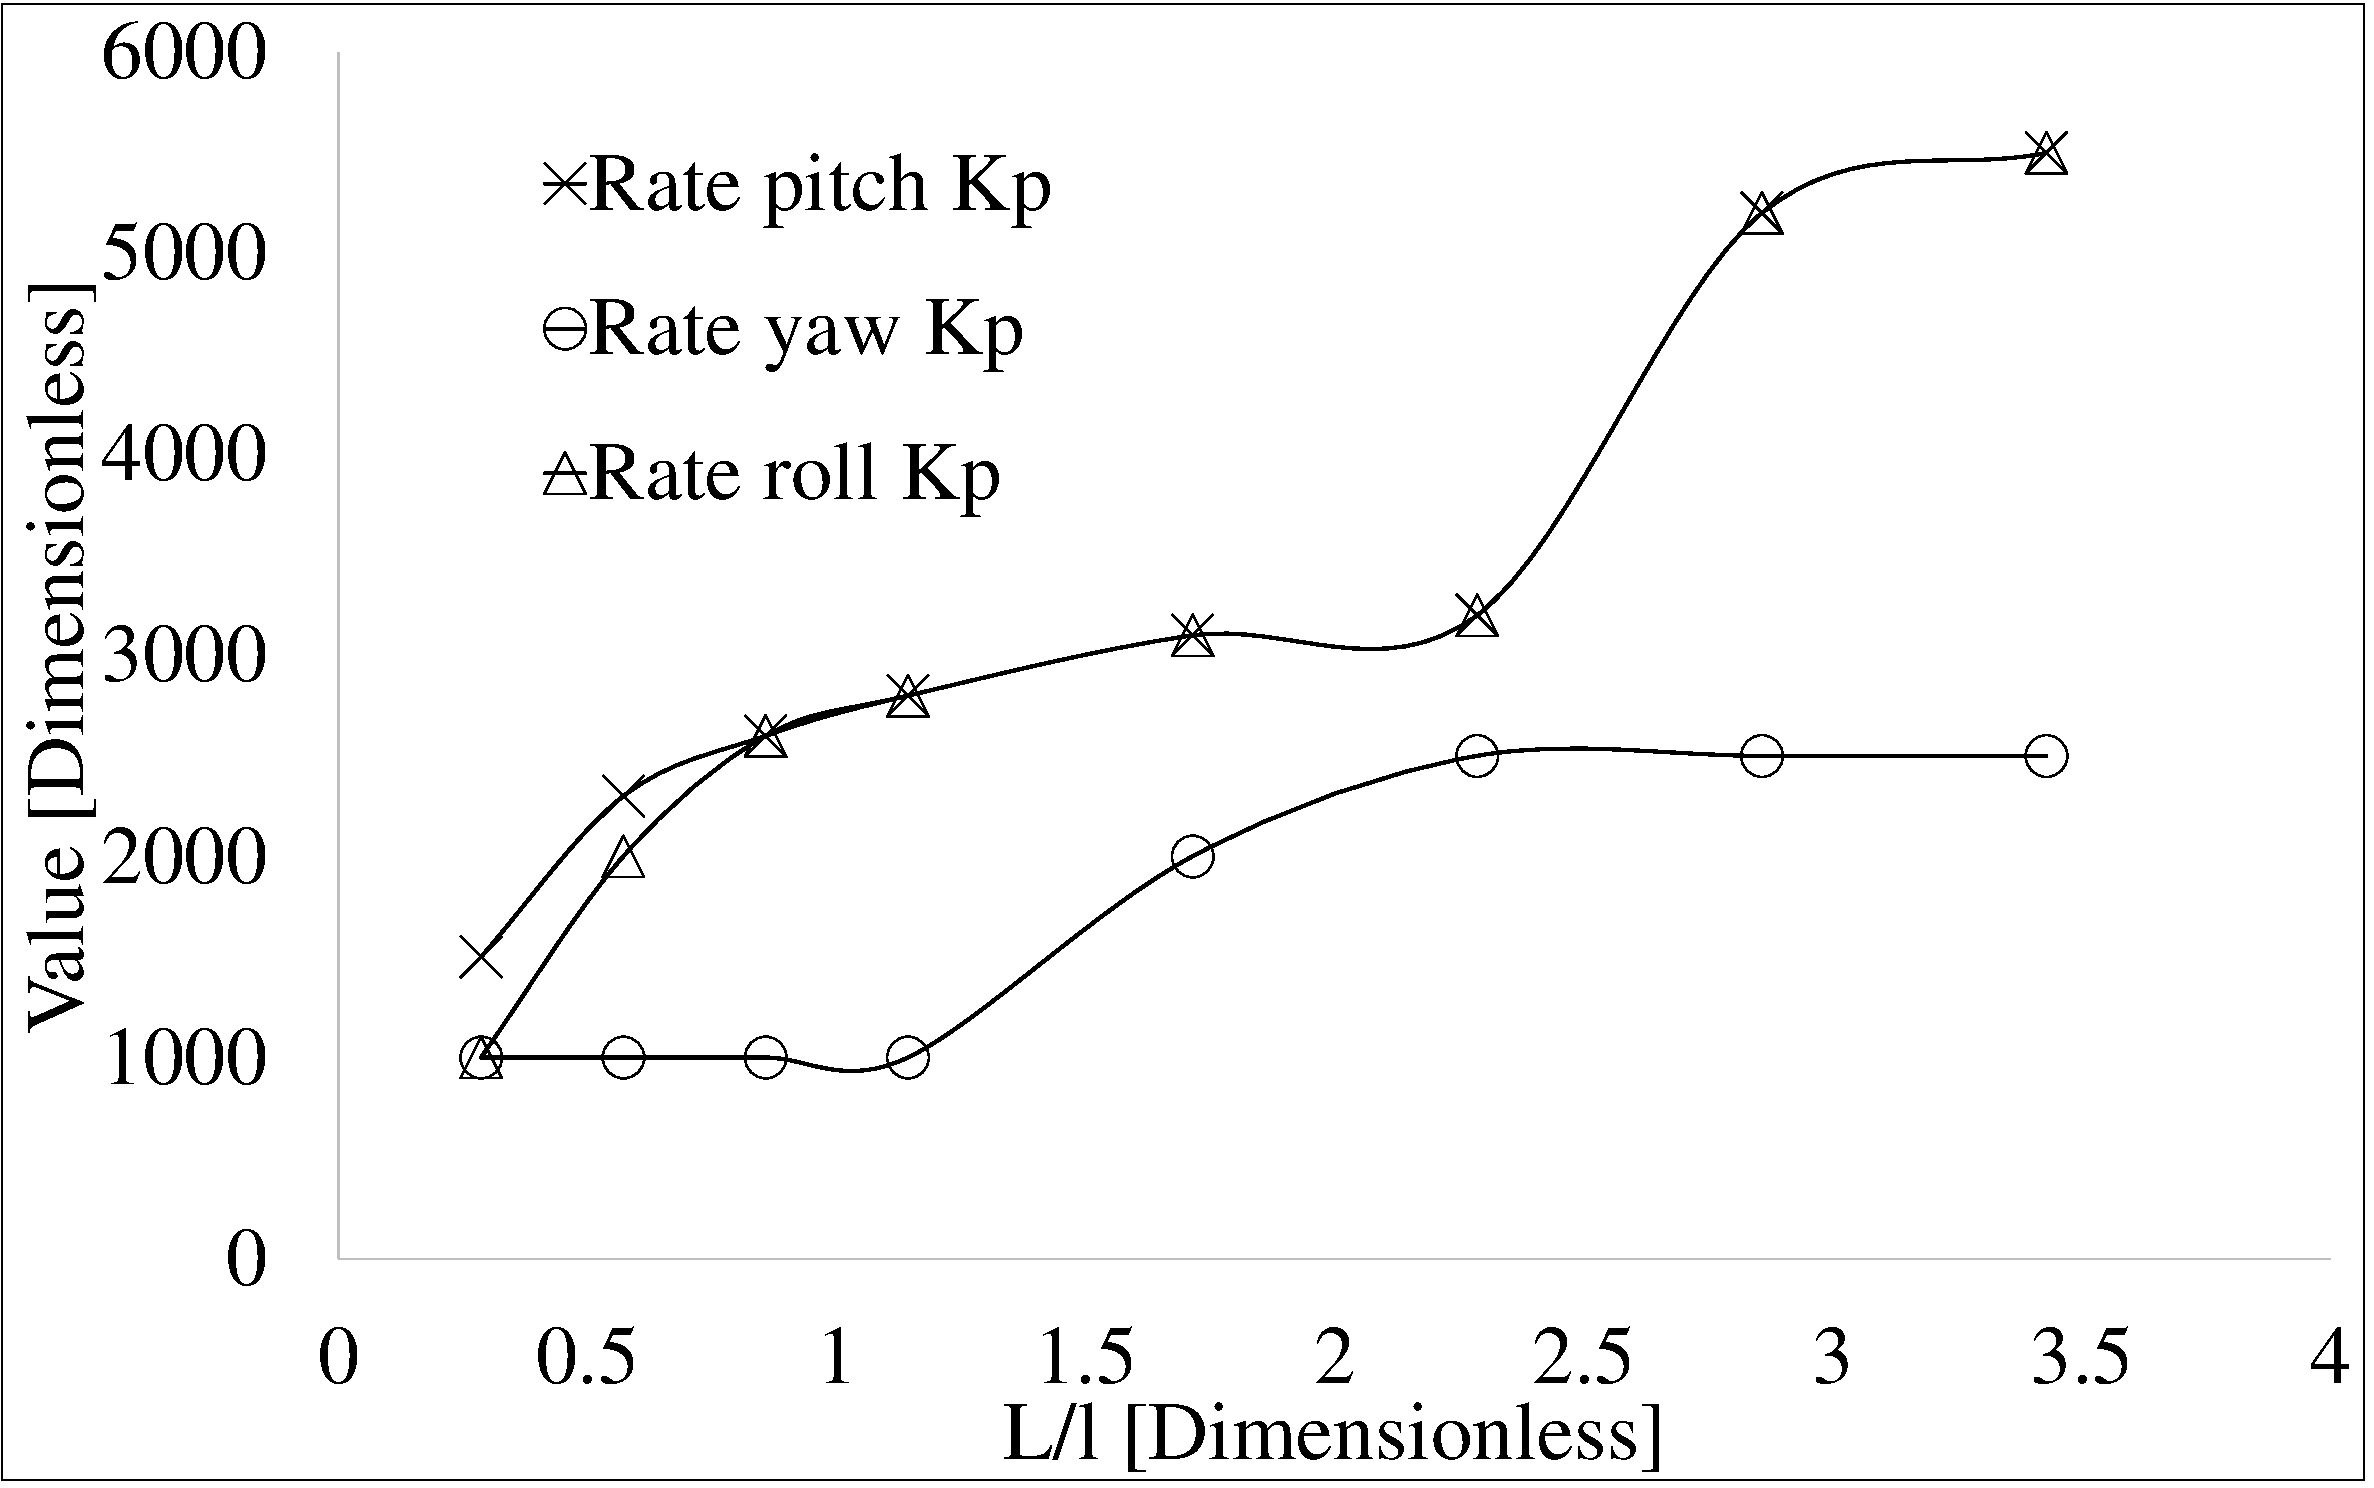
\includegraphics[scale=0.3]{Rate_PID.pdf}
  \caption{(a) Proportional gains of rate controller and \textcolor{red}{(b) attitude proportional gains} as a function of $L/l$}
  \label{fig13}
\end{figure}



\begin{itemize}
\item PID parameter tuning: Anything to do with getting the thing to perch. Talk about everything to do with parameter tuning:
\begin{itemize}
\item Problems with initial test rig and the PID parameters that it gave.(put a picture maybe). Show that motors just shot between 0 and max. Second test rig (p.55)
\item Old vs new PID parameters (some comments on p.55 on use of k$_i$)
\item problems with first tuning rate PID and then angle PID. Say that giving attitude pid a little bit of gain made tuning a lot easier. Also say that with first test rig, cf would stay up during 1 dof tests, but would fall when released into the actual test.
\item Influence of yaw control and why it makes the drone so unstable when it is not correctly tuned. Show pictures of the graphs when it was not correct, and how this differs from the general conception that yaw does not affect roll or pitch. Say also that I had a suspicion with the initial test rig as well, because the roll and pitch balanced on 1 dof tests (p.29), but not when combined without yaw control. Comment that I thought it could be due to loss of info packets.
\item Issues with balancing, monopod support conditions, surface used for tuning (bearings vs slot vs completely flat surface). \textcolor{red}{Talk about how it was very difficult to determine whether the drone was out of balance or that the PID parameters were wrong(kp too high or too low, p.69): Illustrate this with my pictures of changing the orientation of support/using a nominally identical support and the differences in behaviour. Talk about how this balancing issue was dealt with (mass shifting, p.70)}
\item talk about tip of monopod: sharp vs blunt?

\end{itemize} 
\item Results from perching: p.62,63 have stuff on this as well 
\begin{itemize}
\item perch and hover times. Pareto chart. Better a long or short monopod?. Explain why short is more stable (closer to normal flying conditions, ie, just rotating about a mass). Compare perch times of old and new PID parameters?
\item tilt angles (experimental vs model)(impulse,step and ramp. Assess effect of integrator over a sustained disturbance)
\item Maximum yaw rate for each monopod length
\item Having base thrust vs not having base thrust (try different thrust levels)
\item Graph of thrust vs throttle percentage level
\item Talk about PID parameters used during flight with and without perching rig?(They are the same. But maybe putting a bit more K$_I$ helps it from drifting around)
\item Limitations of using such a tiny drone
\item repeatability of tests/trials
\item change in PID parameters with stick length
\end{itemize}
\end{itemize}
Setting the thrust low enough such that drone doesn't fly away
Attitude vs rate mode
Explain how I first intended to tune the drone - DO THIS VERY BRIEFLY TO EXPLAIN MORE EXTENSIVELY ON THE DISCUSSION (following the usual procedure of tuning inside loop first, and outside loop later, each dof separately), and how that did not work (show results/pictures in the results section or here?: Results could be a plot of the different behaviours on different surfaces and 1 dof test rig results vs with no test rig) 


PID loop tuning: Show effects of not having good yaw control (show images of "unexplained" falling), using the initial test rig, and what effect tuning with regular procedures had (tuning in rate mode only and then attitude vs tuning everything at the same time, tuning 1 dof and the others, etc. Show how this gave largely wrong PID parameters only useful for a few surfaces with movement, and not a stationary point). Regular tuning, with 1 dof at a time was justified by the fact that thrust requests were independently added to each motor from each axis. According to this, no yaw control would be necessary to properly tune the drone, but this proved not to be correct.

In my results, I get perching times of 60 min. Since the battery takes 35-40 min to fully charge, it means the drone could be perhaps charged by induction while it is perching, since the charging time is faster than the energy consumption time.

Talk about stick length and sensitivity to unbalanced mass.
\section{Conclusions and future work}
"If I had the knowledge I have now, how would I approach this problem?"
"Future stuff to do"
Good to add some sort of friction/damping mechanism to the end of the monopod such that it is easier to balance it, making it less sensitive to changes in CoG or disturbances.
\begin{itemize}

\item effect of yaw
\item effect of test rig
\item talk about inspiration from omnicube?
\item   \end{itemize}


\bibliographystyle{unsrt}
\bibliography{references}

\pagebreak
\begin{appendices}
\section{Mode shapes and natural frequencies considered}

\end{appendices}
\end{document}